\documentclass[13pt,oneside]{book}
\usepackage[utf8]{inputenc}
\usepackage{url}
\usepackage{listings}
\usepackage{graphicx}

\usepackage{geometry}
\geometry{a4paper, left=20mm, right=20mm, top=20mm, bottom=20mm}
\usepackage[margin=1.2in]{geometry}
\usepackage[toc,page]{appendix}
\usepackage{graphicx}
\usepackage{natbib}
\usepackage{lipsum}
\usepackage{caption}

\begin{document}

\captionsetup[figure]{margin=1.5cm,font=small,labelfont={bf},name={Figure},labelsep=colon,textfont={it}}
\captionsetup[table]{margin=1.5cm,font=small,labelfont={bf},name={Table},labelsep=colon,textfont={it}}
\setlipsumdefault{1}

\begin{titlepage}
\begin{center}
{\LARGE College Of Engineering Trivandrum}\\[3cm]
\linespread{1.2}\huge {\bfseries System Software Lab}\\[3cm]
\linespread{1}

\includegraphics[width=5cm]{img/emblem.jpeg}\\[3cm]
{\Large GOKUL K\\ S5  CSE \\ Roll No:21\\ TVE18CS021 }\\[1cm]


\textit{ }\\[2cm]
Department of Computer Science\\[0.2cm]
\today
\end{center}

\end{titlepage}

\newpage

\begin{frame}{}
    \centering
    \hspace*{-0.5cm}
    $\vcenter{\hbox{
\includegraphics[width=1.5cm]{img/emblem.jpeg}}}$
    $\vcenter{\resizebox{0.95\textwidth}{!}{
        \begin{tabular}{c}
             CS331 - System Software Lab $\cdot$ 2020 $\cdot$   \\
             \hline 
        \end{tabular}
    }}$
\end{frame}
\section*{Cycle 1}
\section*{Expt 5}
\begin{center}
    \Large{Producer Consumer Problem}
\end{center}
\section*{Aim}
\large
To implement the producer-consumer problem using semaphores

\section*{Algorithm} 
    \subsection*{Producer}
    \begin{verbatim}
		1 do
		2 {
		3 // wait until empty > 0 and then decrement empty
		4 wait ( empty ) ;
		5 // acquire lock
		6 wait ( mutex ) ;
		7 /* perform the insert operation in a slot */
		8 // release lock
		9 signal ( mutex ) ;
		10 // increment full
		11 signal ( full ) ;
		12 }
		13 while ( TRUE )
	\end{verbatim}

	\subsection*{Consumer}
	\begin{verbatim}
		1 do
		2 {
		3 // wait until full >0 and then decrement full
		4 wait ( full ) ;
		5 // acquire the lock
		6 wait ( mutex ) ;
		7 /* perform the remove operation in a slot */
		8 // release the lock
		9 signal ( mutex ) ;
		10 // increment empty
		11 signal ( empty ) ;
		12 }
		13 while ( TRUE )
	\end{verbatim}

\section*{Source Code}
\small

\begin{lstlisting}[language=C]
/* Implement the producer-consumer problem using semaphores */
#include <stdio.h>
#include <stdlib.h>

int mutex = 1;
int full = 0, empty = 3, x = 0;

int wait(int);
int signal(int);
void producer();
void consumer();

int wait(int s)
{
	return --s;
}

int signal(int s)
{
	return ++s;
}

void producer()
{
	mutex = wait(mutex);
	full = signal(full);
	empty = wait(empty);
	++x;
	printf("\nItem%d produced", x);
	mutex = signal(mutex);
}

void consumer()
{
	mutex = wait(mutex);
	full = wait(full);
	empty = signal(empty);
	printf("\nItem%d consumed", x);
	--x;
	mutex = signal(mutex);
}

int main()
{
	int n;
	do {
		printf("\n1. Producer\n2. Consumer\n");
		scanf("%d", &n);
		switch(n)
		{
			case 1:
				if(mutex == 1 && empty) producer();
				else printf("\nBuffer overflow");
				break;

			case 2:
				if(mutex == 1 && full) consumer();
				else printf("\nBuffer empty");
				break;
			
			default:
				printf("\nUnknown command");
				exit(0);
		} 
	} while(1);

	return 0;
}
    \end{lstlisting}
    \section*{Output}
    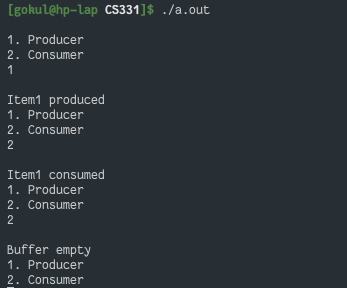
\includegraphics[]{img/p5.png}
    
\Large
\section*{Result}
\large
The producer-consumer problem were solved using semaphores and its output verified
\end{document}